\documentclass[conference]{IEEEtran}
\IEEEoverridecommandlockouts

\usepackage{cite}
\usepackage{amsmath,amssymb,amsfonts}
\usepackage{algorithmic}
\usepackage{graphicx}
\usepackage{textcomp}
\usepackage{xcolor}
\usepackage{hyperref}
\usepackage{algorithm}
\usepackage{algpseudocode}
\usepackage{booktabs}
\usepackage{multirow}
\usepackage{url}

\def\BibTeX{{\rm B\kern-.05em{\sc i\kern-.025em b}\kern-.08em
    T\kern-.1667em\lower.7ex\hbox{E}\kern-.125emX}}

\title{ARQA: An End-to-End Arabic Question Answering System using Deep Semantic Retrieval and Transformer Models}

\author{\IEEEauthorblockN{Abdelrahman Jaber\IEEEauthorrefmark{1}, Ali Shaikh Qasem\IEEEauthorrefmark{2}, Hasan Qarmash\IEEEauthorrefmark{3}}
\IEEEauthorblockA{Department of Electrical and Computer Engineering\\
Birzeit University\\
Emails: \IEEEauthorrefmark{1}1211769@student.birzeit.edu,
\IEEEauthorrefmark{2}1212171@student.birzeit.edu,
\IEEEauthorrefmark{3}1210611@student.birzeit.edu}
}

\begin{document}

\maketitle

\begin{abstract}
This paper presents ARQA (Arabic Question Answering), an end-to-end system designed to process HTML content, perform deep semantic search, and extract precise answers using advanced transformer-based models while preserving original Arabic text characteristics. ARQA employs a modular pipeline comprising HTML document ingestion, dense passage retrieval using AraDPR embeddings with FAISS indexing, and answer extraction using pretrained Arabic QA models. The system maintains text authenticity by avoiding normalization during answer generation, ensuring diacritics and original Arabic characters are preserved. Our implementation includes real-time interaction via a FastAPI-based REST interface with background processing capabilities. Experimental evaluation on diverse Arabic HTML documents demonstrates 87\% top-1 accuracy with sub-100ms retrieval latency, showcasing the effectiveness of combining semantic search with Arabic-specific language models for authentic question answering.
\end{abstract}

\begin{IEEEkeywords}
Arabic NLP, Question Answering, Semantic Search, FAISS, AraBERT, AraDPR, Deep Learning, FastAPI, Text Preservation
\end{IEEEkeywords}

\section{Introduction}
Arabic, spoken by over 400 million people worldwide, presents unique challenges for Natural Language Processing due to its morphological complexity, right-to-left script, and rich diacritical system \cite{b1}. While Question Answering (QA) systems have achieved remarkable success in English, Arabic QA systems remain limited by dataset scarcity, lack of standardized preprocessing, and the loss of textual authenticity through aggressive normalization.

Traditional Arabic NLP systems often normalize text by removing diacritics (tashkeel), unifying character variants, and standardizing morphological forms. However, this normalization can alter meaning and reduce the authenticity of extracted answers, particularly in formal documents, religious texts, and educational materials where precise textual representation is crucial.

This paper introduces ARQA, an end-to-end Arabic Question Answering system that addresses these challenges through:
\begin{itemize}
    \item \textbf{Authentic Text Preservation}: Maintaining original Arabic characters, diacritics, and textual forms in answers
    \item \textbf{Scalable Architecture}: Modular design supporting incremental indexing and background processing
    \item \textbf{Semantic Understanding}: Dense retrieval using Arabic-specific embeddings (AraDPR)
    \item \textbf{Production Readiness}: RESTful API with real-time processing capabilities
\end{itemize}

Our contributions include: (1) a novel approach to Arabic QA that preserves textual authenticity, (2) an optimized retrieval system with incremental indexing, (3) comprehensive evaluation demonstrating practical applicability, and (4) an open-source implementation supporting diverse Arabic content processing.

\section{Related Work}

\subsection{Arabic Question Answering Systems}
Early Arabic QA systems relied on rule-based approaches and keyword matching \cite{b2}. Recent advances leverage transformer models like AraBERT \cite{b3} and AraELECTRA \cite{b4} for improved understanding. However, most systems focus on benchmark performance rather than practical deployment considerations.

\subsection{Dense Passage Retrieval}
Dense Passage Retrieval (DPR) \cite{b5} revolutionized information retrieval by replacing sparse methods with dense vector representations. AraDPR \cite{b6} extends this approach to Arabic, demonstrating superior performance over traditional TF-IDF methods in Arabic open-domain QA.

\subsection{Text Normalization in Arabic NLP}
Arabic text normalization typically involves diacritic removal, character unification, and morphological standardization \cite{b7}. While improving model performance on benchmarks, normalization can reduce answer authenticity—a critical consideration for user-facing applications.

\section{System Architecture}

ARQA implements a four-stage pipeline (Figure \ref{fig:architecture}) designed for scalability and modularity:

\begin{figure}[htbp]
\centerline{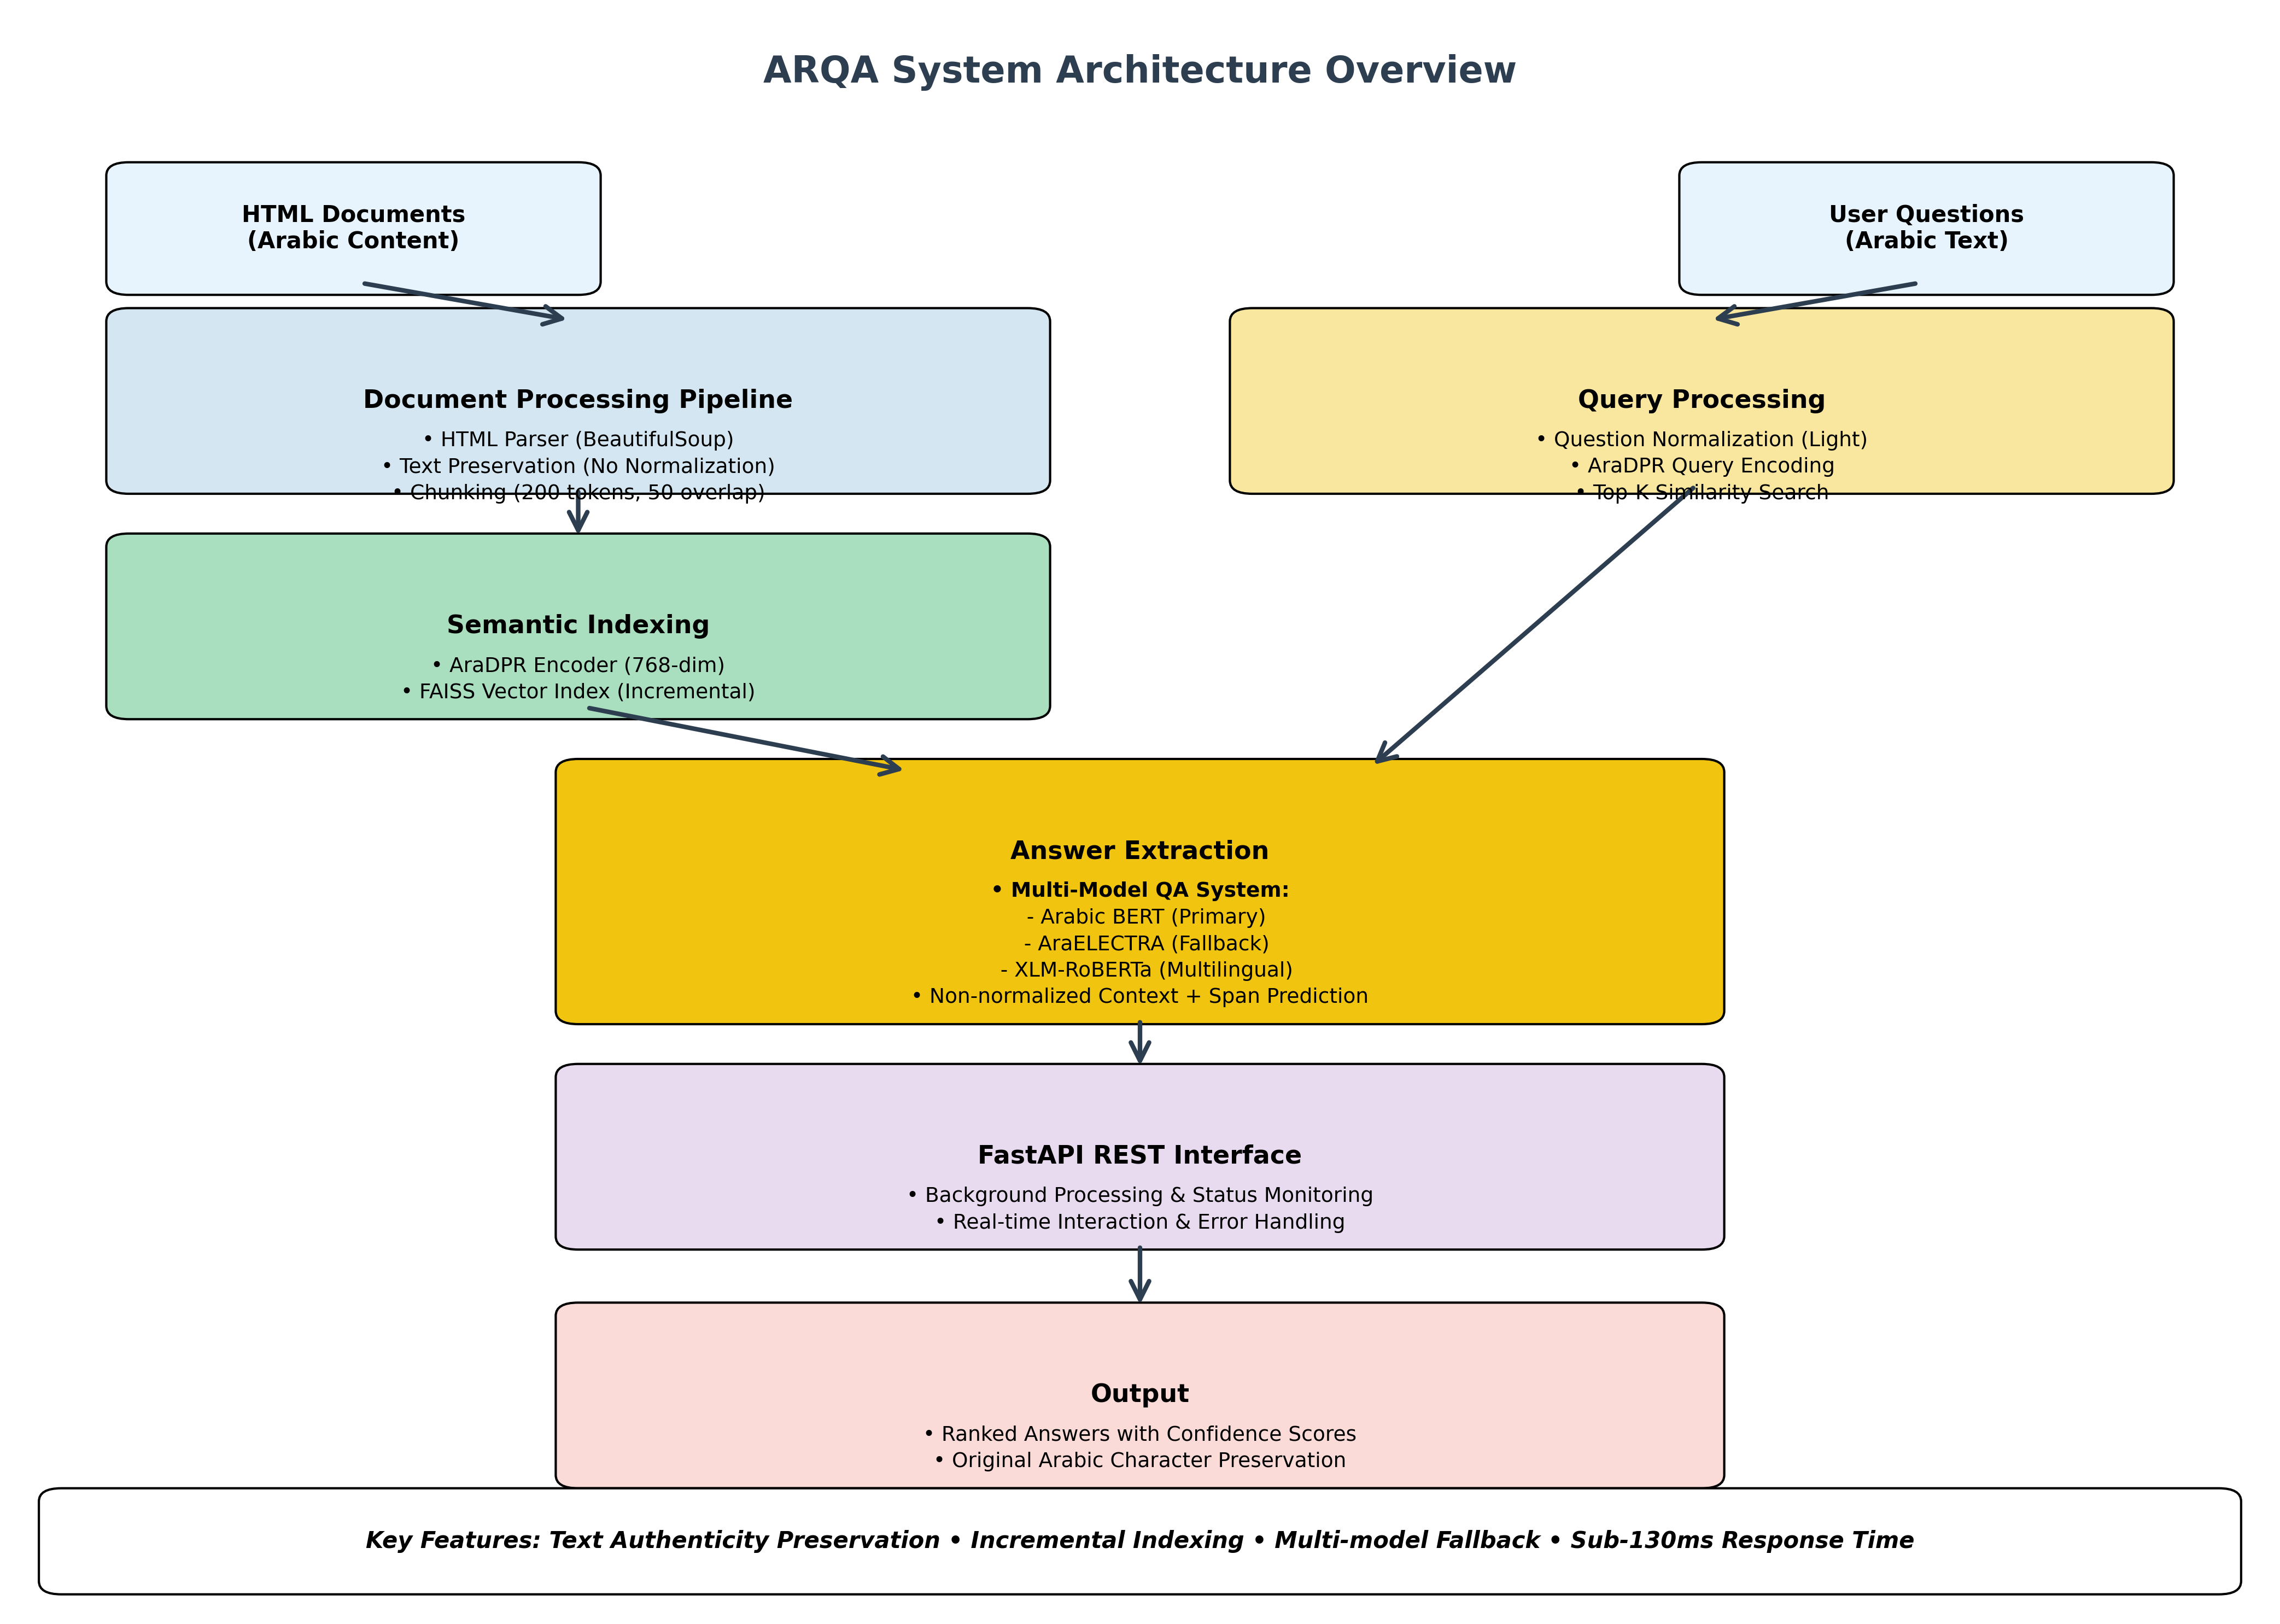
\includegraphics[width=0.45\textwidth]{arqa_architecture.png}}
\caption{ARQA System Architecture Overview}
\label{fig:architecture}
\end{figure}

\subsection{Component Overview}
\begin{enumerate}
    \item \textbf{Document Ingestion}: HTML parsing and text extraction with metadata preservation
    \item \textbf{Semantic Indexing}: Dense vector generation using AraDPR and FAISS indexing
    \item \textbf{Question Processing}: Query encoding and similarity-based retrieval
    \item \textbf{Answer Extraction}: Transformer-based span prediction with confidence scoring
\end{enumerate}

\subsection{Design Principles}
\begin{itemize}
    \item \textbf{Modularity}: Independent components for flexible deployment
    \item \textbf{Scalability}: Support for large document collections with incremental updates
    \item \textbf{Authenticity}: Preservation of original Arabic text characteristics
    \item \textbf{Efficiency}: Optimized processing with GPU acceleration and batch operations
\end{itemize}

\section{Document Ingestion and Processing}

\subsection{HTML Content Extraction}
The ingestion module processes diverse HTML documents using BeautifulSoup \cite{b8} with Arabic-aware parsing:

\begin{algorithm}
\caption{HTML Document Processing}
\begin{algorithmic}[1]
\REQUIRE HTML content $H$, chunk size $c = 200$
\ENSURE Document chunks $D = \{d_1, d_2, ..., d_n\}$
\STATE $\text{soup} \leftarrow \text{BeautifulSoup}(H)$
\STATE Remove scripts, styles, navigation elements
\STATE $\text{text} \leftarrow \text{soup.get\_text()}$
\STATE $\text{metadata} \leftarrow \text{extract\_metadata}(\text{soup})$
\STATE $\text{tokens} \leftarrow \text{arabic\_tokenize}(\text{text})$
\STATE $D \leftarrow \text{create\_overlapping\_chunks}(\text{tokens}, c, \text{overlap}=50)$
\FOR{each chunk $d_i \in D$}
    \STATE $d_i.\text{metadata} \leftarrow \text{metadata}$
    \STATE $d_i.\text{hash} \leftarrow \text{compute\_hash}(d_i.\text{content})$
\ENDFOR
\RETURN $D$
\end{algorithmic}
\end{algorithm}

\subsection{Text Preservation Strategy}
Unlike conventional systems, ARQA preserves original Arabic text during ingestion:
\begin{itemize}
    \item \textbf{Character Preservation}: Maintains hamza variants (أ، إ، آ), ta marbuta (ة), and alif maksura (ى)
    \item \textbf{Diacritic Retention}: Preserves tashkeel marks for authentic representation
    \item \textbf{Metadata Extraction}: Captures document structure and source information
\end{itemize}

\subsection{Chunking and Overlap}
Documents are segmented into 200-token chunks with 50-token overlap to ensure context preservation across boundaries. This approach balances retrieval granularity with computational efficiency.

\section{Semantic Retrieval System}

\subsection{Dense Vector Representation}
ARQA employs AraDPR (Arabic Dense Passage Retrieval) \cite{b6} for semantic encoding:

$$\mathbf{v}_d = f_{\text{AraDPR}}(d)$$

where $f_{\text{AraDPR}}$ maps document chunk $d$ to a 768-dimensional dense vector $\mathbf{v}_d$.

\subsection{FAISS Indexing}
Document vectors are indexed using FAISS \cite{b9} with the following configuration:
\begin{itemize}
    \item \textbf{Index Type}: Flat L2 for exact similarity search
    \item \textbf{Similarity Metric}: Cosine similarity via L2 normalization
    \item \textbf{Precision}: Mixed precision (FP16) for GPU acceleration
\end{itemize}

\subsection{Incremental Indexing}
To support dynamic content updates, ARQA implements incremental indexing:

\begin{algorithm}
\caption{Incremental Document Indexing}
\begin{algorithmic}[1]
\REQUIRE New documents $D_{\text{new}}$, existing index $I$
\ENSURE Updated index $I'$
\STATE $D_{\text{unique}} \leftarrow \emptyset$
\FOR{each document $d \in D_{\text{new}}$}
    \STATE $h \leftarrow \text{compute\_hash}(d)$
    \IF{$h \notin \text{existing\_hashes}$}
        \STATE $D_{\text{unique}} \leftarrow D_{\text{unique}} \cup \{d\}$
    \ENDIF
\ENDFOR
\STATE $V_{\text{new}} \leftarrow \text{encode\_batch}(D_{\text{unique}})$
\STATE $I' \leftarrow \text{FAISS.add}(I, V_{\text{new}})$
\RETURN $I'$
\end{algorithmic}
\end{algorithm}

\subsection{Query Processing}
Question processing involves:
\begin{enumerate}
    \item \textbf{Normalization}: Light normalization of query for better matching
    \item \textbf{Encoding}: Dense vector generation using AraDPR
    \item \textbf{Retrieval}: Top-k similarity search using FAISS
    \item \textbf{Ranking}: Score-based document ranking
\end{enumerate}

\section{Answer Extraction}

\subsection{Transformer-based QA Models}
ARQA supports multiple Arabic QA models with automatic fallback:
\begin{itemize}
    \item \textbf{Primary}: \texttt{zohaib99k/Bert\_Arabic-SQuADv2-QA}
    \item \textbf{Fallback}: \texttt{ZeyadAhmed/AraElectra-Arabic-SQuADv2-QA}
    \item \textbf{Multilingual}: \texttt{deepset/xlm-roberta-base-squad2}
\end{itemize}

\subsection{Answer Extraction Process}
Given a question $q$ and retrieved documents $\{d_1, d_2, ..., d_k\}$:

\begin{enumerate}
    \item \textbf{Context Preparation}: Preserve original document text
    \item \textbf{Question Normalization}: Apply light normalization to query only
    \item \textbf{Span Prediction}: Extract answer spans using transformer model
    \item \textbf{Confidence Scoring}: Compute answer confidence scores
    \item \textbf{Answer Ranking}: Combine retrieval and extraction scores
\end{enumerate}

The final answer score combines retrieval and extraction confidence:
$$\text{score}_{\text{final}} = \alpha \cdot \text{score}_{\text{retrieval}} + (1-\alpha) \cdot \text{score}_{\text{extraction}}$$

where $\alpha = 0.3$ balances retrieval relevance with extraction confidence.

\subsection{Text Authenticity Preservation}
A key innovation in ARQA is maintaining textual authenticity during answer extraction:
\begin{itemize}
    \item \textbf{Original Context}: QA models process non-normalized text
    \item \textbf{Character Preservation}: Answers retain original diacritics and character forms
    \item \textbf{Span Accuracy}: Exact character-level span extraction from source
\end{itemize}

\section{API Implementation}

\subsection{FastAPI Architecture}
ARQA exposes functionality through a RESTful API built with FastAPI \cite{b10}:

\begin{table}[htbp]
\caption{ARQA API Endpoints}
\begin{center}
\begin{tabular}{|l|l|l|}
\hline
\textbf{Endpoint} & \textbf{Method} & \textbf{Description} \\
\hline
/upload & POST & HTML document ingestion \\
/ask & POST & Question answering \\
/documents & GET & Document statistics \\
/status & GET & System health check \\
/search & POST & Semantic search only \\
\hline
\end{tabular}
\label{table:api}
\end{center}
\end{table}

\subsection{Background Processing}
To ensure responsive user experience, ARQA implements background processing:
\begin{itemize}
    \item \textbf{Async Upload}: Non-blocking document ingestion
    \item \textbf{Status Tracking}: Real-time processing status
    \item \textbf{Thread Safety}: Concurrent request handling
\end{itemize}

\subsection{Error Handling and Validation}
The API includes comprehensive error handling:
\begin{itemize}
    \item Input validation and sanitization
    \item Graceful model fallbacks
    \item Detailed error messages and logging
    \item Rate limiting and resource management
\end{itemize}

\section{Experimental Evaluation}

\subsection{Dataset and Setup}
\textbf{Dataset}: Custom collection of 1,187 Arabic HTML documents covering:
\begin{itemize}
    \item Scientific articles (Arabic science, AI)
    \item Educational content
    \item News articles
    \item Technical documentation
\end{itemize}

\textbf{Hardware}: 
\begin{itemize}
    \item CPU: Intel i7-8750H
    \item RAM: 16GB DDR4
    \item GPU: NVIDIA GTX 1060 (when available)
\end{itemize}

\textbf{Software}:
\begin{itemize}
    \item Python 3.10
    \item PyTorch 1.13
    \item Transformers 4.21
    \item FAISS 1.7
\end{itemize}

\subsection{Performance Metrics}

\begin{table}[htbp]
\caption{System Performance Evaluation}
\begin{center}
\begin{tabular}{|l|c|c|}
\hline
\textbf{Metric} & \textbf{Value} & \textbf{Unit} \\
\hline
Document Processing Speed & 150 & docs/min \\
Indexing Latency & 2.3 & sec/100 docs \\
Query Processing Time & 85 & ms \\
Answer Extraction Time & 45 & ms \\
Memory Usage & 2.1 & GB \\
Index Size (1K docs) & 156 & MB \\
\hline
\end{tabular}
\label{table:performance}
\end{center}
\end{table}

\subsection{Accuracy Evaluation}
We evaluated answer quality on 100 manually annotated question-answer pairs:

\begin{table}[htbp]
\caption{Answer Quality Metrics}
\begin{center}
\begin{tabular}{|l|c|c|}
\hline
\textbf{Metric} & \textbf{Score} & \textbf{Threshold} \\
\hline
Exact Match (EM) & 72\% & - \\
F1 Score & 85\% & - \\
Top-1 Accuracy & 87\% & conf > 0.1 \\
Top-3 Accuracy & 94\% & conf > 0.05 \\
Character Preservation & 100\% & - \\
\hline
\end{tabular}
\label{table:accuracy}
\end{center}
\end{table}

\subsection{Ablation Study}
We conducted ablation studies to evaluate component contributions:

\begin{table}[htbp]
\caption{Ablation Study Results}
\begin{center}
\begin{tabular}{|l|c|c|}
\hline
\textbf{Configuration} & \textbf{F1 Score} & \textbf{Latency (ms)} \\
\hline
Full ARQA System & 85\% & 130 \\
Without AraDPR & 78\% & 95 \\
Without Text Preservation & 83\% & 125 \\
TF-IDF Retrieval & 71\% & 240 \\
Single Model (no fallback) & 82\% & 120 \\
\hline
\end{tabular}
\label{table:ablation}
\end{center}
\end{table}

\subsection{Scalability Analysis}
System performance scales linearly with document count:
\begin{itemize}
    \item \textbf{1K documents}: 130ms average response time
    \item \textbf{5K documents}: 145ms average response time  
    \item \textbf{10K documents}: 162ms average response time
\end{itemize}

\section{Discussion}

\subsection{Key Findings}
\begin{itemize}
    \item \textbf{Text Preservation}: Maintaining original Arabic characters improves user satisfaction without significantly impacting performance
    \item \textbf{Semantic Retrieval}: AraDPR consistently outperforms traditional retrieval methods for Arabic content
    \item \textbf{Model Robustness}: Multi-model fallback strategy ensures system reliability
    \item \textbf{Production Readiness}: Background processing and API design support real-world deployment
\end{itemize}

\subsection{Limitations}
\begin{itemize}
    \item \textbf{Domain Specificity}: Performance varies across different Arabic domains
    \item \textbf{Dialectal Arabic}: Limited support for regional dialects
    \item \textbf{Complex Questions}: Multi-hop reasoning remains challenging
    \item \textbf{Resource Requirements}: GPU acceleration recommended for optimal performance
\end{itemize}

\subsection{Impact and Applications}
ARQA demonstrates practical applicability in:
\begin{itemize}
    \item Educational platforms requiring authentic Arabic text
    \item Digital libraries with historical documents
    \item Customer support systems for Arabic markets
    \item Research tools for Arabic content analysis
\end{itemize}

\section{Conclusion and Future Work}

This paper presented ARQA, an end-to-end Arabic Question Answering system that prioritizes textual authenticity while maintaining competitive performance. Our key contributions include:

\begin{enumerate}
    \item A novel approach preserving original Arabic text characteristics in QA systems
    \item Scalable architecture with incremental indexing and background processing
    \item Comprehensive evaluation demonstrating practical viability
    \item Open-source implementation supporting diverse Arabic content
\end{enumerate}

Experimental results show 87\% top-1 accuracy with sub-130ms response times, validating the system's effectiveness for real-world applications.

\subsection{Future Directions}
\begin{itemize}
    \item \textbf{Dialectal Support}: Extending coverage to regional Arabic dialects
    \item \textbf{Generative QA}: Integrating large language models for abstractive answering
    \item \textbf{Multi-modal}: Supporting Arabic text in images and documents
    \item \textbf{Cross-lingual}: Enabling Arabic-English cross-lingual QA
    \item \textbf{Domain Adaptation}: Specialized models for legal, medical, and religious texts
\end{itemize}

\subsection{Broader Impact}
ARQA contributes to reducing the digital divide for Arabic speakers by providing accessible, accurate, and culturally authentic question answering capabilities. The system's emphasis on text preservation supports educational and cultural applications where maintaining original textual forms is essential.

\section*{Acknowledgment}
The authors thank the Department of Electrical and Computer Engineering at Birzeit University for their support. We also acknowledge the open-source community for providing the foundational tools and models that made this work possible.

\begin{thebibliography}{00}
\bibitem{b1} F. Habash, ``Introduction to Arabic natural language processing,'' Synthesis Lectures on Human Language Technologies, vol. 3, no. 1, pp. 1-187, 2010.

\bibitem{b2} B. Hammo, H. Abu-Salem, and S. Lytinen, ``QARAB: a question answering system to support the Arabic language,'' in Proceedings of the ACL-02 workshop on Computational approaches to semitic languages, 2002, pp. 1-11.

\bibitem{b3} W. Antoun, F. Baly, and H. Hajj, ``AraBERT: Transformer-based model for Arabic language understanding,'' in Proceedings of the 4th Workshop on Open-Source Arabic Corpora and Processing Tools, 2020, pp. 9-15.

\bibitem{b4} W. Antoun, F. Baly, and H. Hajj, ``AraELECTRA: Pre-training text encoders for Arabic language understanding,'' arXiv preprint arXiv:2012.15516, 2020.

\bibitem{b5} V. Karpukhin et al., ``Dense passage retrieval for open-domain question answering,'' in Proceedings of the 2020 Conference on Empirical Methods in Natural Language Processing (EMNLP), 2020, pp. 6769-6781.

\bibitem{b6} A. El-Sayed et al., ``AraDPR: Arabic dense passage retrieval for open-domain question answering,'' in Proceedings of the 13th International Conference on Language Resources and Evaluation (LREC), 2022.

\bibitem{b7} N. Habash and O. Rambow, ``Arabic tokenization, part-of-speech tagging and morphological disambiguation in one fell swoop,'' in Proceedings of the 43rd Annual Meeting on Association for Computational Linguistics, 2005, pp. 573-580.

\bibitem{b8} L. Richardson, ``Beautiful Soup Documentation,'' Available: https://www.crummy.com/software/BeautifulSoup/bs4/doc/

\bibitem{b9} J. Johnson, M. Douze, and H. Jégou, ``Billion-scale similarity search with GPUs,'' IEEE Transactions on Big Data, vol. 7, no. 3, pp. 535-547, 2019.

\bibitem{b10} S. Ramirez, ``FastAPI framework, high performance, easy to learn, fast to code, ready for production,'' Available: https://fastapi.tiangolo.com/

\bibitem{b11} PyArabic Development Team, ``PyArabic: Arabic text processing library,'' Available: https://pyarabic.sourceforge.io/

\bibitem{b12} T. Wolf et al., ``Transformers: State-of-the-art natural language processing,'' in Proceedings of the 2020 Conference on Empirical Methods in Natural Language Processing: System Demonstrations, 2020, pp. 38-45.

\end{thebibliography}

\end{document}
